\section{NumPy}
\subsection{Introduction}
NumPy (Numerical Python) is a library for performing mathematical functions and operations on large multidimensional arrays. It provides:
\begin{itemize}
    \item \textbf{Speed}: Utilizes optimized C code, replacing slow standard Python \texttt{for} loops.
    \item \textbf{Vectorization}: Array-based operations are executed element-wise automatically.
    \item \textbf{Broadcasting}: Implicitly expands arrays of different shapes during arithmetic calculations.
\end{itemize}

\subsection{Creation of n-dimensional Arrays (\texttt{ndarray})}
The \texttt{ndarray} is a homogeneous data structure where each dimension is called an \textit{axis}.
\begin{itemize}
    \item \texttt{arr.ndim}: Number of dimensions.
    \item \texttt{arr.shape}: Tuple representing the size of each dimension. (rows, cols)
    \item \texttt{arr.dtype}: Data type of the array elements (e.g., \texttt{np.float64}, \texttt{np.int32}).
    \item \texttt{arr.astype(dtype)}: Returns a copy of the array cast to a specific type.
\end{itemize}

\subsubsection{Array Creation Methods}
\lstinputlisting[language=Python]{code/np_array_creation.py}


\resizebox{\columnwidth}{!}{
\begin{tabular}{l|l}
\textbf{Funktion} & \textbf{Resultat} \\ \hline
\texttt{np.ones((2,2))} & \texttt{array([[1., 1.], [1., 1.]])} \\
\texttt{np.ones\_like(arr1)} & \texttt{array([1, 1, 1])} \\
\texttt{np.zeros((2,2))} & \texttt{array([[0., 0.], [0., 0.]])} \\
\texttt{np.zeros\_like(arr1)} & \texttt{array([0, 0, 0])} \\
\texttt{np.full((2,2), 7.0)} & \texttt{array([[7., 7.], [7., 7.]])} \\
\texttt{np.full\_like(arr1, 7)} & \texttt{array([7, 7, 7])} \\
\texttt{np.eye(2)} & \texttt{array([[1., 0.], [0., 1.]])} \\
\texttt{np.linspace(0, 1, 5)} & \texttt{array([0., 0.25, 0.5, 0.75, 1.])} \\
\texttt{np.arange(0, 4, 0.5)} & \texttt{array([0, 0.5, 1, 1.5, 2, 2.5, 3, 3.5])} \\
\texttt{np.logspace(0, 1, 4)} & \texttt{array([1., 2.1544, 4.6416, 10.])} \\
\texttt{np.random.randn(3)} & \texttt{array([0.7576, 0.0135, -0.8934])} \\
\texttt{np.random.randint(0,10,3)} & \texttt{array([0, 5, 4])} \\
\end{tabular}}\medbreak

In \texttt{arange} è possibile inserire uno \texttt{step} negativo, per creare un array decrescente.

\crd{Attenzione al fatto che \texttt{end} è escluso dall'array,} se si vuole includere: (\texttt{end} $\pm$ \texttt{step})

\columnbreak

\subsection{Element Access}
\begin{itemize}
    \item \textbf{Indexing}: Axes are separated by commas within brackets (e.g., \texttt{arr[row, col]}).
    \item \textbf{Slicing}: Follows the \texttt{[start:end:step]} syntax across multiple
     axes. Slicing returns a \textbf{view}; modifications affect the original array. 
     Use \texttt{.copy()} to create an independent duplicate.
     \crd{END not included!}
    \item \textbf{Boolean Slicing}: Extracts subsets where a condition is \texttt{True} (e.g., \texttt{arr[arr > 5]}).
\end{itemize}


\textbf{Examples:}

\begin{center}
    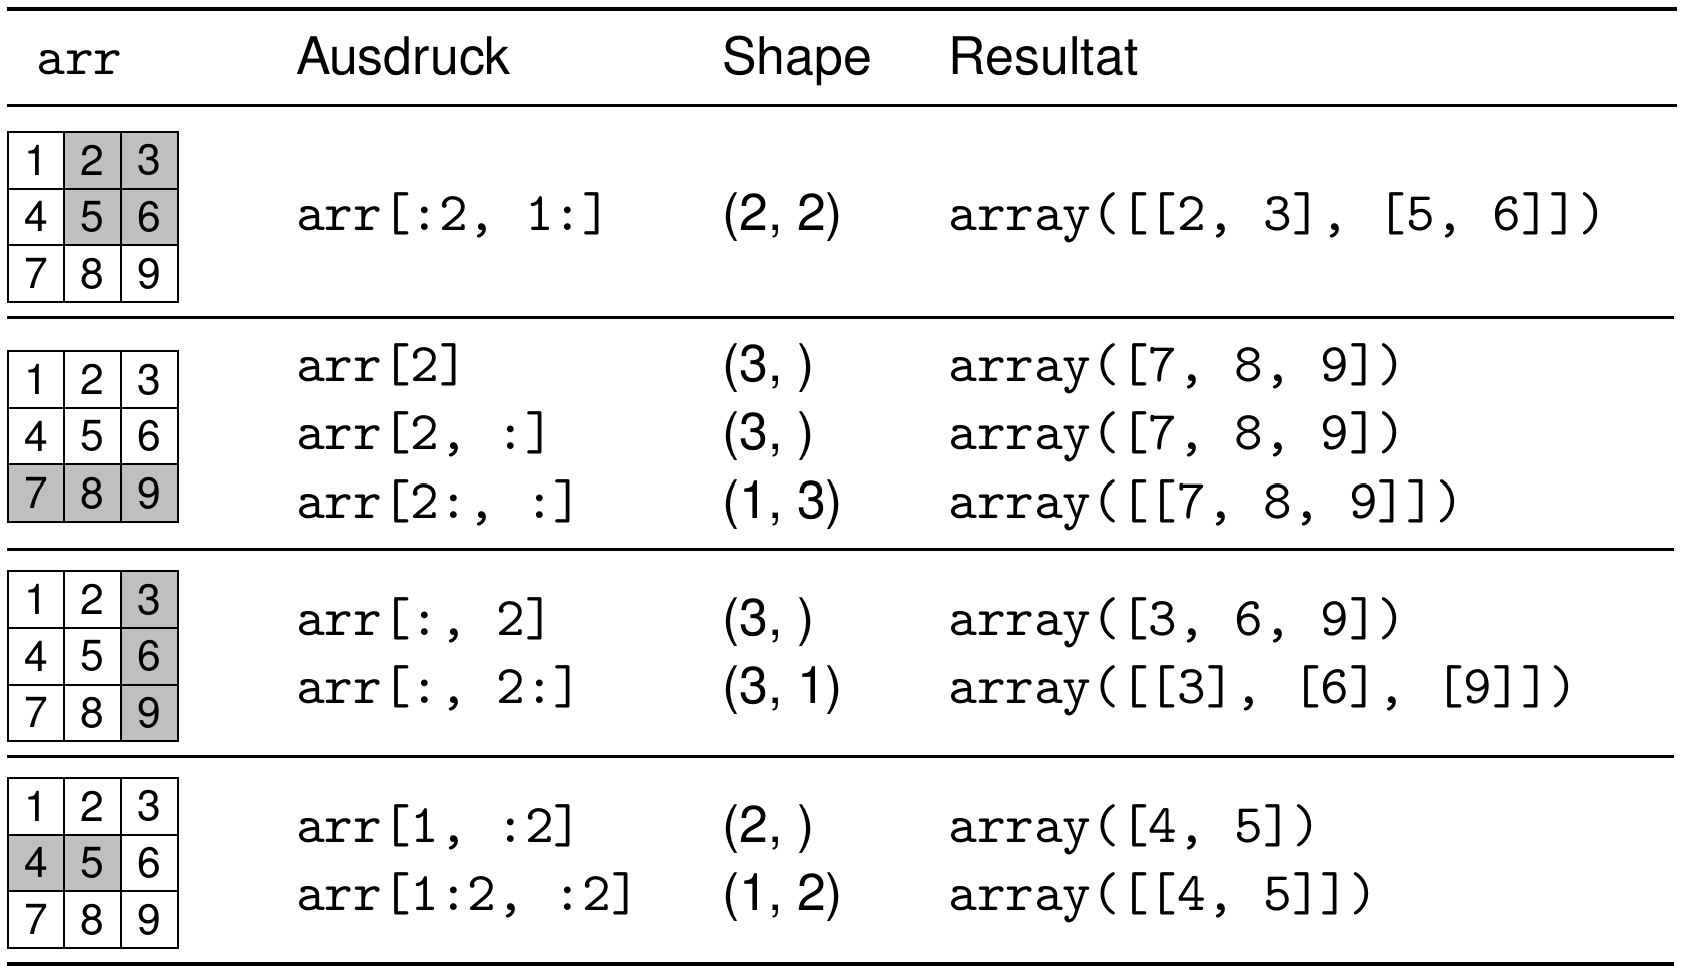
\includegraphics[width=0.7\linewidth]{images/slicing.png}
\end{center}

\begin{minipage}{0.45\columnwidth}
    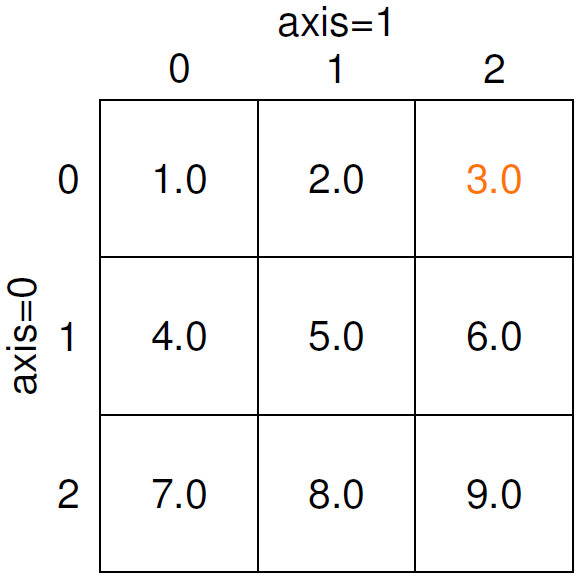
\includegraphics[width=\linewidth]{images/indizierung3.png}
\end{minipage}\hfill
\begin{minipage}{0.45\columnwidth}
    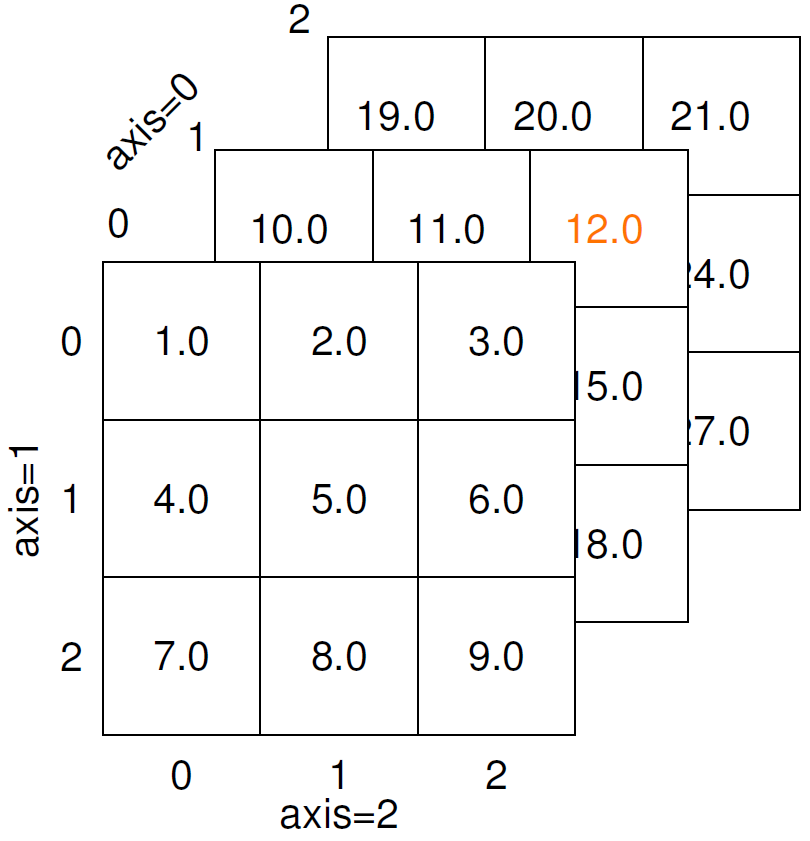
\includegraphics[width=\linewidth]{images/indizierung4.png}
\end{minipage}

The axes will always change when adding/removing dimesnions

\subsection{Broadcasting}
To perform operations on arrays of different shapes, NumPy automatically broadcasts the smaller array:
\begin{enumerate}
    \item Dimensions are inserted on the left until the number of dimensions (\texttt{ndim}) matches.
    \item Dimensions of size 1 are stretched to match the corresponding dimension of the other array.
    \item If sizes differ and neither is 1, a \texttt{ValueError} is raised.
\end{enumerate}

\subsection{Array Manipulation}
\subsubsection{Concatenation and Stacking}
\lstinputlisting[language=Python]{code/np_concatenation.py}


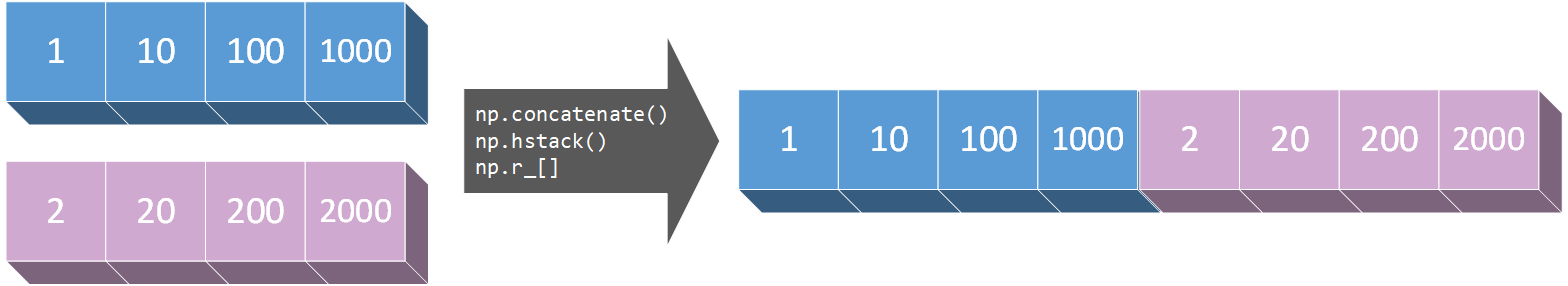
\includegraphics[width=\linewidth]{images/stacking_1D_1D.png}
\begin{center}
    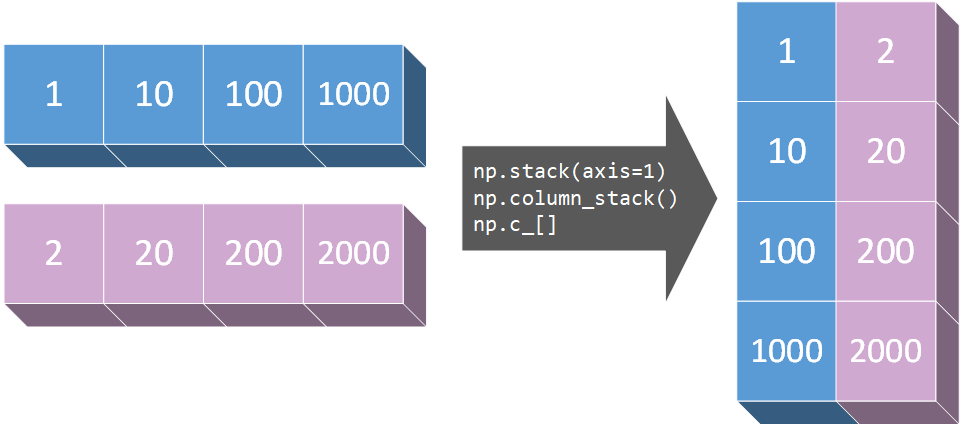
\includegraphics[width=0.7\linewidth]{images/stacking_1D_2D_spaltenweise.png}
\end{center}

\subsubsection{Dimension Changes}
\lstinputlisting[language=Python]{code/np_dimesnions.py}

Please note: arr.reshape(-1) only creates a view, not an actual copy


\subsection{Mathematical Functions}
NumPy provides vectorized universal functions (ufuncs) such as: \texttt{np.exp()}, \texttt{np.sin()}, \texttt{np.abs()}, \texttt{np.mean()}, \texttt{np.max()}, \texttt{np.std()}, and \texttt{np.cumsum()}.

% --- SUBSECTION: ADVANCED CONCATENATION & LINEAR ALGEBRA ---
\subsection{Concatenation}
\textbf{MATLAB-like Concatenation:}

\begin{itemize}
    \item \texttt{np.r\_}: Concatenates along the first axis (row-wise). It supports slice objects and individual values.
    \item \textit{Example:} \texttt{x = np.r\_[1:5, 15, 20:50:10]} $\rightarrow$ \texttt{[1, 2, 3, 4, 15, 20, 30, 40]}
    \item \texttt{np.c\_}: Concatenates along the second axis (column-wise). Ideal for creating column vectors.
    \item \textit{Example:} \texttt{y = np.c\_[0:3]} $\rightarrow$ \texttt{[[0], [1], [2]]}
\end{itemize}

\subsection{NumPy Linear Algebra: Multiplication Summary}

\subsubsection{Scalar and Vector Products}
\begin{itemize}
    \item \textbf{np.inner(a, b):} Best for the \textbf{Scalar Product} (inner product) of two vectors. 
    \begin{itemize}
        \item \textit{When to use:} Use it when you specifically want the inner product of vectors. It is clearer than \texttt{dot()} because it is restricted to this specific operation.
        \item \textit{Example:} \texttt{v1 = [1, 2]; v2 = [3, 4] $\to$ 1*3 + 2*4 = 11}.
    \end{itemize}
    
    \item \textbf{np.outer(a, b):} Computes the \textbf{Dyadic Product} (outer product).
    \begin{itemize}
        \item \textit{When to use:} Use it to create a matrix from two vectors (Column Vector $\times$ Row Vector).
        \item \textit{Example:} \texttt{v1 = [1, 2]; v2 = [3, 4] $\to$ [[3, 4], [6, 8]]}.
    \end{itemize}
\end{itemize}

\subsubsection{Matrix Multiplication: @ vs np.dot()}
While both perform standard matrix multiplication for 2D arrays, they behave differently for higher-dimensional tensors ($n > 2$).

\begin{itemize}
    \item \textbf{The @ Operator (np.matmul):} The standard for \textbf{Matrix Multiplication}.
    \begin{itemize}
        \item \textit{Behavior ($n > 2$):} It treats the array as a 'stack' of matrices and multiplies them across their final two dimensions.
        \item \textit{Recommendation:} This is the preferred method for standard matrix multiplication in modern Python (3.5+).
    \end{itemize}
    
    \item \textbf{np.dot(a, b):}
    \begin{itemize}
        \item \textit{Behavior ($n > 2$):} It calculates the sum of products across the \textbf{last} dimension of $a$ and the \textbf{penultimate} dimension of $b$.
        \item \textit{Result:} It effectively multiplies the first row of $a$ by EVERY column in each subsequent matrix of $b$, leading to a much larger resulting shape.
    \end{itemize}
\end{itemize}

\cor{Usually always use the \texttt{@} operator}
\subsubsection{Comparison Example ($n > 2$)}
\begin{lstlisting}[language=Python]
a = np.ones((2, 3, 3))
b = np.ones((2, 3, 3))

# Result: (2, 3, 3) -> Multiplies stacks independently
res_matmul = a @ b 

# Result: (2, 3, 2, 3) -> Multiplies every row by every column
res_dot = np.dot(a, b)     
\end{lstlisting}
